\documentclass[12pt]{article}
\usepackage{pagestyle}

\begin{document}
\thispagestyle{empty}

{\scshape ML } \hfill {\scshape \large Lecture 0 - Probability part} \hfill {\scshape 18.02.2024}
 
\smallskip
\hrule
\bigskip

\section{Probability}

\subsection{Types of probability}
Probability can be divided into two main types : \textbf{objective} and \textbf{subjective}. \\
The most common form of objective probability is \textbf{frequentist probability}. 
\begin{definition}[Frequentist probability]
    Probability is only a property of a (hypothetical) repeated experiments.
\end{definition}

The most common form of subjective probability is \textbf{Bayesian probability}.
\begin{definition}[Bayesian probability]
    Probability is an expression of our uncertainty and of our beliefs.
\end{definition}

\subsection{Basic concepts}
There are 4 core concepts in probability theory: \textbf{sample space}, \textbf{event space}, \textbf{probability function}, \textbf{random variable}.

\subsection{Sample space $\Omega$}

\begin{definition}[Sample space]
    The set of all possible outcomes of an experiment. Denoted by $\Omega$. For example $\Omega = \{H, T\}$ for a coin flip.
\end{definition}

\begin{definition}[Discrete sample space]
    A sample space is discrete if it is finite or countably infinite. E.g. $\Omega = \{1, 2, 3, 4, 5, 6\}$ for a die roll.
\end{definition}

\begin{definition}[Continuous sample space]
    A sample space is continuous if it is uncountably infinite. E.g. $\Omega = \mathbb{R}$ for a continuous random variable.
\end{definition}

The examples summarized:
\begin{itemize}[leftmargin=*, noitemsep]
    \item $\Omega = \{1, 2, 3, 4, 5, 6\}$ for a die roll.
    \item $\Omega = \{H, T\}$ for two coin flips.
    \item $\Omega = \mathbb{R}$ for a continuous random variable.
\end{itemize}

\subsection{Event space}

\begin{definition}[Event space $E$]
    For a \textit{discrete} sample space the corresponding event space is a the set of all subsets of the sample space AKA the \textit{power set}. For a \textit{continuous} sample space the event space is the set of all intervals.
\end{definition}

\begin{definition}[Event]
    An event is something which has a probability. This can include \textit{atomic events} or \textit{compound events}.    
\end{definition}

\begin{definition}[Atomic event]
    An atomic event is a single outcome of an experiment. For example $\{1\}$ for a die roll.
\end{definition}

\begin{definition}[Compound event]
    A compound event is an event with more than one sample point, such as the probability of rolling a 1 or a 2 in the case of a die roll.
\end{definition}

For example in the case of a die roll: 
\begin{itemize}[leftmargin=*, noitemsep]
    \item sample space $\Omega = \{1, 2, 3, 4, 5, 6\}$
    \item event space $E = \{\{\}, \{1\}, \{2\}, \{3\}, \ldots, \{1, 2\}, \ldots, \{1, 2, 3, 4, 5, 6\}\}$
\end{itemize}

\subsection{Random variables}

\begin{definition}[Random variable $X$]
    Intuitively a random variable is a way to describe events. It takes a sample space and describes some set of events.
\end{definition}

Some examples of random variables assuming $X$ = sample space of a die roll:
\begin{itemize}[leftmargin=*, noitemsep]
    \item $X = 1$ for the event of rolling a 1.
    \item $X > 3$ for the event of rolling a number greater than 3.
    \item $X = 2 \text{ or } 3$ for the event of rolling a 2 or a 3.
\end{itemize}

\begin{definition}[Probability function $P$]
    A probability function is a function which takes a random variable (e.g. $X = 3$) and returns a probability, generally in decimal form between 0 and 1 (inclusive).
\end{definition}

Some examples of probability functions assuming $X$ = sample space of a die roll:
\begin{itemize}[leftmargin=*, noitemsep]
    \item $p(X = 1) = \frac{1}{6}$
    \item $p(X > 3) = \frac{1}{2}$
    \item $p(X = 2 \text{ or } 3) = \frac{2}{6} = \frac{1}{3}$
\end{itemize}

\begin{definition}[Probability function of regular variable $p(X = x)$]
    Probability functions can either be functions of well-defined events or functions of regular variables.
\end{definition}

If we have an event space with only two atomic events $\{-1, 1\}$ then we can define a probability function for a variable $x$ representing these events as follows:
\[
    p(X = x) = p(X) = p(x) = \begin{cases}
        \frac{1}{4} & \text{if } x = -1 \\
        \frac{3}{4} & \text{if } x = 1
    \end{cases}  
\]

In the case we have boolean random variables the notation is as follows: 
\begin{align*}
    p(X) & = p(X = \text{true}) \\ 
    p(\neg X) & = p(X = \text{false})  
\end{align*}

\subsection{Probability vs Probability density}

In the case of a discrete sample space we have probabilities assigned to each atomic event. For example 50\% for a coin flip. In the case of a continuous sample space we have a probability density function (pdf) which gives the probability of a random variable being in a certain interval. For example the probability of a random variable being between 0 and 1.

\begin{definition}[Probability density]
    Probability density expresses the probability of a random variable being in a certain continous interval.
\end{definition}

Some notes on probability density:
\begin{itemize}[leftmargin=*, noitemsep]
    \item In the case of a continuous sample space the probability of a random variable being in a single point is 0.
    \item The probability of a random variable being in a certain interval is the integral of the probability density function over that interval.
\end{itemize}

\subsection{Joint probability}

\begin{definition}[Joint probability $p(X, Y)$]
    Joint probability is the probability of two random variables being in a certain state at the same time. It can either be \textit{instantiated} or \textit{uninstantiated}.
\end{definition}

To explain this we use an example teeth health and age, as usual first there is the sample space: 
\begin{align*}
    \text{Age} & = \{\text{young}, \text{teen}, \text{old}\}  \\
    \text{Teeth} & = \{\text{healthy}, \text{unhealthy}, \text{fake}\}
\end{align*}

The sample space then consits of all possible combinations of these two random variables, which makes up 9 pairs. We expresses the uninstantiated probability distribution for all these combinations as follows 
\[
    p(\text{Age}, \text{Teeth})  
\]

\begin{definition}[Instantiated joint probability $p(X = x, Y = y)$]
    Instantiated joint probability is the probability of two random variables being in a certain specific state at the same time.
\end{definition}

For example $p(\text{Age} = \text{young}, \text{Teeth} = \text{healthy})$.

\subsection{Marginal probability}

\begin{definition}[Marginal probability $p(X)$]
The marginal probability of a random variable is the probability of that random variable being in a certain state. Calculating the marginal probability is called \textit{marginalizing out} because we sum over the rows or columns of the variable we are interested in and write the results in the margins.
\end{definition}

The formula for marginal probability is as follows:
\[
    p(X) = \sum_{y \in Y} p(X, Y = y)  
\]

Applying this to the example below for the marginal probability that $p(\text{Age} = \text{old})$ we get:
\[
    p(\text{A} = \text{o}) = p(\text{o}, \text{T} = \text{h}) + p(\text{o}, \text{T} = \text{u}) + p(\text{o}, \text{T} = \text{f}) = \frac{1}{18} + \frac{1}{18} + \frac{3}{18} = \frac{5}{18} 
\] 
\begin{figure}[h!]
    \centering
    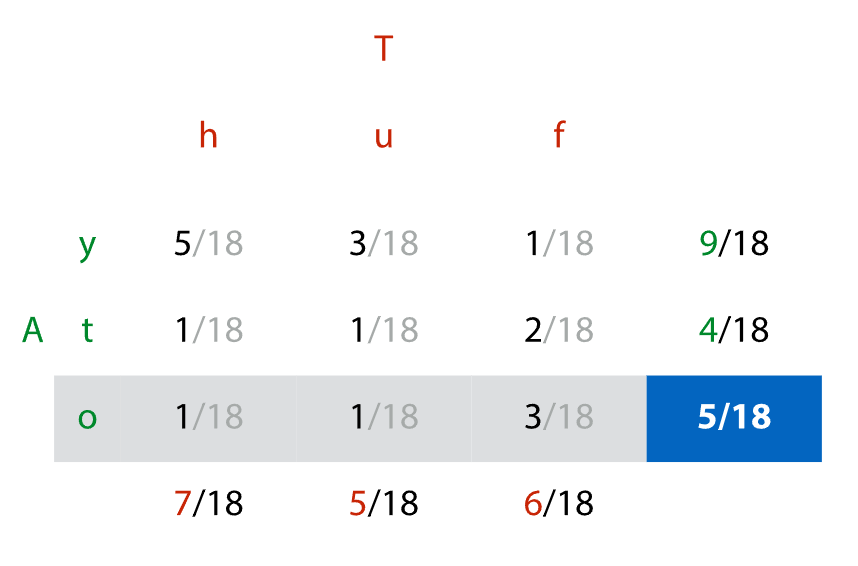
\includegraphics[width=0.4\textwidth]{assets/marginalprob.png}
    \caption{Marginal probability}
\end{figure}

\subsection{Conditional probability}

\begin{definition}[Conditional probability $p(X\mid Y)$]
    Conditional probability is the probability of a random variable being in a certain state given that another random variable is in a certain state.
\end{definition}

The formula for conditional probability is as follows:
\[
    p(X = x\mid Y = y) = \frac{p(X = x, Y = y)}{\underbrace{\sum_{x'} p(X = x', Y = y)}_{\text{marginal probability}}} = \frac{p(x, y)}{p(y)} \quad p(X = x) \Leftrightarrow p(x)
\]  

A useful formula form this is the one for joint probability as a function of conditional probability and marginal probability:
\[
    p(x, y) = p(x\mid y) p(y)  
\]

Applying the formula for the conditional probability to the example below we get:
\[
    P(\text T = \text f \mid  \text A = \text y) = \frac{p(f, y)}{p(y)} = \frac{1}{9}    
\]

\subsubsection*{Marginalizing out in higher dimensions}

Broadly speaking marginalizing out in higher dimensions for continous distributions is done similar to the discrete case but we use integrals instead of sums. 

\begin{figure}[h!]
    \centering
    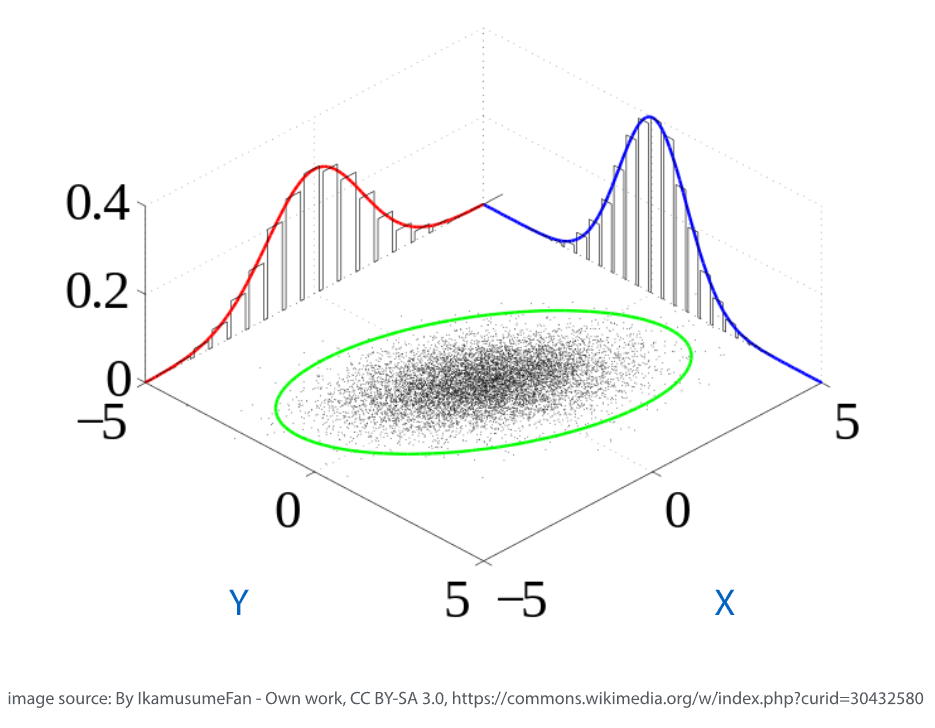
\includegraphics[width=0.4\textwidth]{assets/hdmarginalprob.png}
    \caption{marginal probability in higher dimensions}
\end{figure}

\subsection{Independence}

\begin{definition}[Independence]
    If two variables X and Y are independent then knowing Y will not change what we know about X. 
\end{definition}

Formally we can express independence as follows:
\begin{align*}
    & p(X\mid Y) = p(X) \\
    \rightarrow & P(X, Y)  = p(X)p(Y)
\end{align*}

\begin{definition}[Conditional independence]    
    Conditional independence means that two variables can be dependent, \text{but} their dependence is entirely explained by a third variable. 
\end{definition}

Formally $X$ and $Y$ are conditionally independent given $Z$ if:
\[
    p(X, Y\mid Z) = p(X\mid Z)p(Y\mid Z)  
\]

As an example let say 
\begin{align*}
    X & = \text{Alice is home in time for dinner} \\
    Y & = \text{Bob is home in time for dinner} \\
    Z & = \text{A monster attacks the city}
\end{align*}

We assume in most cases the the time when Alice or Bob are home for dinner are independent. So knowing the time for Alice tells us nothing about the time for Bob and vv. But if a monster attacks the city then we assume this effects the time of \text{both} Alice and Bob, thus given that a monster attacks the city if we observe the time for Alice or Bob we \text{can} infer the time for the other person. \\ 
The key takeaways from this being that: 
\begin{itemize}
    \item Any dependence between $X$ and $Y$ is entirely explained by the monster attacking the city. Formally 
    \[
        p(X, Y\mid Z) = p(X\mid Z)p(Y\mid Z)
    \]
    \item If we know that the monster attacked the city then any further information about $X$ or $Y$ is redundant. Formally 
    \[
        p(X\mid Y, Z) = p(X\mid Z)
    \]
\end{itemize}

\subsection{Bayes' rule}

\begin{definition}[Inversion problem]
    The inversion problem is the problem of finding the probability of some hidden cause given an observed effect. 
\end{definition}

An example would be the situation where we call a restaurant to place an order yet noone picks up the phone. 
One line of reasoning you might follow is to 
\begin{enumerate}[leftmargin=*, noitemsep]
    \item Assume that the restaurant burned down 
    \item Since the restaurant burned down there is a high probability noone would answer the phone
\end{enumerate}
Here we are reasoning from the cause (the restaurant burned down) to the effect (noone answers the phone). More formally we are essentially saying that 
\[
    p(\text{noone answers the phone}\mid \text{restaurant burned down}) 
\]
is high and this lines up with our observation.\\

Though by the inversion problem we are interested in the opposite, we already know that noone answered the phone and we want to know the probability that the restaurant burned down. This is where Bayes' rule comes in. Which is the probability of the cause given the effect. Formally 
\[
    p(\text{cause} \mid \text{effect}) = \frac{1}{p(\text{effect})} p(\text{effect} \mid \text{cause}) p(\text{cause})
\]

\subsubsection*{Bayes Example}

Situation: Alice is late for dinner, we don't know if this is because a monster attacked the city, but we also can't say a monster didn't attack. So lets try and figure out the probability that a monster attacked (cause $m$) the city given that Alice is late for dinner (effect $a$).
\begin{align*}
    p(m\mid a) & = \frac{p(a\mid m)p(m)}{p(a)} \\ 
    & = \frac{p(a\mid m )p(m)}{\underbrace{p(a\mid t)p(t)}_{\text{traffic}} + \underbrace{p(a\mid m)p(m)}_{\text{monster}} + \underbrace{p(a\mid s)p(s)}_{\text{snowfall}} } 
\end{align*}

Here we assume there are 3 possible causes to Alice being late, namely traffic, the monster attacking and snowfall. The denominator is the sum marginalizing out over all possible causes.

\subsection{Expectation}

\begin{definition}[Expectation]
    The expectation (expected value) is a way of expressing what you can expect to gain from a random process.
\end{definition}

Formally for a given outcome function $f(x)$ and a probability function $p(x)$ the expectation is given by:
\[
    E[f(x)] = \sum_{x} f(x)p(x)= \int_{x} f(x)p(x)dx
\] 
Equivelantly we can also think of it as the sum of a finite list of $x_1, x_2, \ldots, x_n$ outcomes with corresponding probabilities $p_1, p_2, \ldots, p_n$:
\[
    E[f(x)] = x_1p_1 + x_2p_2 + \cdots + x_n p_n  
\]

\subsubsection*{A die roll bet}
Say for a bet you roll $n \leq 3$ you pay the corresponding amount of dollars. If you roll $n > 3$ you get the corresponding amount of dollars. We can define the expected value for this as 
\[
    E[X] = (-3)\frac{1}{6} + (-2)\frac{1}{6} + (-1)\frac{1}{6} + (4)\frac{1}{6} + (5)\frac{1}{6} + (6)\frac{1}{6} = 1.5 
\]

\subsubsection*{Rules}

There are some basic rules for manipulating expectations, all based mostly just on the same rules for manipulating sums and integrals since thats all expectations are formally.

\begin{align*}
    E[c] & = c \\ 
    E[cf(x)] & = cE[f(x)] \\
    E[c + f(x)] & = c + E[f(x)] \\ 
    E[f(x) + g(x)] & = E[f(x)] + E[g(x)] \\
\end{align*}

\subsection{Common probability distributions}

\subsubsection*{Bernoulli distribution}

\begin{definition}[Bernoulli distribution]
    Any distribution with two outcomes. The probability of the first outcome is $p$ and the probability of the second outcome is $1 - p$. 
\end{definition}

Some examples include: 
\begin{itemize}[leftmargin=*, noitemsep]
    \item heads or tails
    \item guilty or innocent 
    \item positive negative
\end{itemize}

\subsubsection*{Categorial distribution}

\begin{definition}[Categorial distribution]
    Any distribution with some finite number (>2) of $n$ outcomes. Where the probabilities of each outcome sum to 1. That is $p_1 + p_2 + \cdots + p_n = 1$. Hence we only need $n - 1$ probabilities to describe the distribution.
\end{definition}

Some examples include:
\begin{itemize}[leftmargin=*, noitemsep]
    \item which team wins the next world cup 
    \item hair color of a random person in ireland  
\end{itemize}

\subsubsection*{Normal distribution}

\begin{definition}[Normal distribution]
    The normal distribution is a continuous distribution with a bell-shaped curve. It is defined by two parameters, the mean $\mu$ and the standard deviation $\sigma$.   
\end{definition}

The parameters express 
\begin{itemize}[leftmargin=*, noitemsep]
    \item $\mu$ the center of the distribution
    \item $\sigma$ the spread of the distribution
    \item $\sigma^2$ the variance of the distribution
\end{itemize}

The distribution is good at expressing things that have a definite scale no matter the scale we are working at. For example no matter how many humans we look at most people will have a height clustered around the mean with fewer and fewer people having heights further and further from the mean.

\subsubsection*{Multivariate normal distribution}

\begin{definition}[Multivariate normal distribution]
    The multivariate normal distribution is a generalization of the normal distribution to higher dimensions.
\end{definition}

\end{document}